\documentclass{article}

\setlength{\parindent}{0 pt}

\usepackage{fullpage, xspace, enumitem, graphicx}

\usepackage[pdfborder={.25 .25 .25}]{hyperref}

\urlstyle{rm}

\usepackage{microtype}

\newcommand{\blob}{\textbf{Blob}\xspace}
\newcommand{\blobs}{\textbf{Blob}s\xspace}
\newcommand{\valuex}{\textbf{Value}\xspace}
\newcommand{\valuexs}{\textbf{Value}s\xspace}
\newcommand{\object}{\textbf{Object}\xspace}
\newcommand{\objects}{\textbf{Object}s\xspace}
\newcommand{\encode}{\textbf{Encode}\xspace}
\newcommand{\thunk}{\textbf{Thunk}\xspace}
\newcommand{\thunks}{\textbf{Thunk}s\xspace}
\newcommand{\blobthunk}{\textbf{Blob Thunk}\xspace}
\newcommand{\blobthunks}{\textbf{Blob Thunk}s\xspace}
\newcommand{\treethunk}{\textbf{Tree Thunk}\xspace}
\newcommand{\treethunks}{\textbf{Tree Thunk}s\xspace}
\newcommand{\encodes}{\textbf{Encode}s\xspace}
\newcommand{\name}{\textbf{Name}\xspace}
\newcommand{\names}{\textbf{Name}s\xspace}
\newcommand{\tree}{\textbf{Tree}\xspace}
\newcommand{\trees}{\textbf{Tree}s\xspace}
\newcommand{\pathx}{\textbf{Path}\xspace}
\newcommand{\pathxs}{\textbf{Path}s\xspace}
\newcommand{\bs}{\vspace{\baselineskip}}

\begin{document}
%\thispagestyle{empty}

\textbf{Computation in the Fixpoint OS}\newline
Yuhan Deng, Sadjad Fouladi, Keith Winstein, with commentary by Amit Levy (last updated: 1/14/2022)

\bs

Fixpoint is a ``deterministic operating system'' that roughly follows
the design of the SICP
\href{https://mitpress.mit.edu/sites/default/files/sicp/full-text/book/book-Z-H-27.html#\%_sec_4.2.2}{``Interpreter
  with Lazy Evaluation''}. The data model is similar to a Git
repository, one that can also represent computational relations
between content-addressed objects: e.g., ``blob \texttt{<x>} is the
output of computation \texttt{<y>} given tree \texttt{<z>} as input.''
The intention is to support a range of applications, including
pre-existing \textsc{posix} programs, and for the OS to provide
``determinism-safety'': program execution is referentially
transparent, and irreproducibility is considered an OS bug, even
across different computers.\footnote{Not \emph{everything} can be
referentially transparent---IO has to happen somewhere. Fixpoint does have a
context where IO is permitted, akin to an ``unsafe'' block in Rust,
but the intention is to let programmers and users constrain and
delimit the non-deterministic parts of a program, rather than allowing
unrestricted IO to happen anywhere.} We envision cloud-computing
providers offering ``computation as a service'': the customer provides
a description of a computation, and the provider returns the answer
for a fee, perhaps backed by an insurance policy that guarantees
correctness.

%\vspace{0.5\baselineskip}
%{\Large \textbf{1. Types}}

\section{Types}

\subsection{\objects, \valuexs, and \thunks}

The basic type is an \object. Each \object is immutable, has one canonical representation, and is either:

\begin{itemize}[itemsep=0pt]
\item a \valuex, which is either:
\begin{itemize}[itemsep=0pt]
  \item a \blob: a vector of bytes, or

  \item a \tree: a vector of entries, each containing:

    \begin{enumerate}[topsep=0pt, itemsep=0pt]
    \item a \name, and

    \item a boolean indicating whether the entry is ``strict'' or ``lazy,''
    \end{enumerate}
\end{itemize}

\item or a \thunk, which represents a particular \valuex by specifying
  a way to compute it. Internally, a \thunk contains the \name of an \encode.
\end{itemize}

\object identity is defined by equality of the canonical representation.

\subsection{\names}

A \name is a string that identifies a particular \object by means of an unambiguous
reference, either:
    \begin{itemize}[itemsep=0pt]
    \item a ``canonical name'': the \textsc{sha-256} hash of the \object's canonical representation,
    \item a ``local name'': a locally generated unique ID that identifies an \object, or
    \item a ``literal'': the canonical representation of the \object itself.
    \end{itemize}

\names are opaque; two \names that identify the same \object are equivalent for purposes of computation.

\subsection{\encodes}

An \encode\footnote{For ``Explicit Named Computation On Data or
\encodes.''} is a \tree that describes the application of a function
to inputs, producing an \object as output. The first entry specifies
the resource limits at runtime (e.g., maximum pages of mutable memory). The second entry
species the function, which is either:
\begin{itemize}[itemsep=0pt]
\item A \blob that contains a Wasm module, or
\item An \encode.
\end{itemize}

At evaluation-time, the function can read any ``accessible \valuex'' in
the \encode---which means any strict entry of the \encode, and any
strict entry of an ``accessible'' \tree. A lazy entry refers to an
\object that the function can include in its output (as a lazy or
strict entry), without being able to read its contents.\footnote{This
can support functions that do short-circuit evaluation,
e.g. ``\texttt{if}'' or ``\texttt{and},'' while retaining the
referential transparency of \thunks for their corresponding
\valuexs. That is, without full-blown \texttt{fexprs}.}

\bs

We chose Wasm as the basic representation of computation because (1)
LLVM can compile into it, which lets many existing programs and
languages be used, (2) it can run at near-native speed, both in terms
of throughput ($>85\%$ of native) and invocation latency ($<$~100~ns),
and (3) it's possible to guarantee that computations are
deterministic, at least within a microarchitectural
family\footnote{One of the few sources of nondeterminism in Wasm is
the freedom for the underlying microarchitecture, e.g.~x86-64 or \textsc{arm}, to represent floating-point NaNs
with different bitwise representations.}

\section{State}

The system maintains several global mappings:
\begin{itemize}[itemsep=0pt]
\item The ``storage'' maps a \name to the contents of the corresponding \object.

\item The ``memoization cache'' maps a \thunk to the \name of an \object that represents
  a reduction of the original \thunk. This target may be either another \thunk, or the referred-to \valuex.

\item The ``trace cache'' maps a \name to a human-readable string.
\end{itemize}

\section{Operations}

\begin{quote}
\begin{quote}
\textit{It has been said that the principal function of an operating system
is to define a number of different names for the same object, so that it
can  busy  itself  keeping  track of the relationship between all of the
different names.} (David Clark, 1982\footnote{\href{https://www.rfc-editor.org/rfc/rfc814.html}{RFC 814}.})
\end{quote}
\end{quote}

\subsection{Forcing}

``Forcing'' is an function from \objects to \valuexs:

\begin{itemize}[itemsep=0pt]
\item Forcing a \blob is the identity operation.

\item Forcing a \tree forces each of its strict entries, replacing the
  entry's \name field with the \name of the resulting \valuex.

\item Forcing a \thunk recursively reduces it to its referred-to \valuex.
\end{itemize}

\subsection{Reducing a \thunk (one step)}

``Reducing'' a \thunk transforms it to another \thunk or to the
eventual \valuex. To do this, the system will:
\begin{itemize}[itemsep=0pt]
\item retrieve a memoized reduction from the memoization cache, or
\item compute the reduction, by:
  \begin{enumerate}[topsep=0pt, itemsep=0pt]
  \item evaluating the \encode that the \thunk names,
  \item returning the \encode's output \object, and
  \item optionally inserting an entry into the memoization cache from the \thunk to the output \object.
  \end{enumerate}
\end{itemize}

\subsection{Forcing a \thunk}

Forcing a \thunk means:
\begin{enumerate}[itemsep=0pt]
\item reducing it, and
\item if the resulting \object is a \thunk, forcing that \thunk in turn.
\end{enumerate}

\subsection{Evaluating an \encode}

To evaluate an \encode, the system will:
\begin{enumerate}[itemsep=0pt]
\item force the \encode itself, transforming each strict entry into a \valuex
\item run the Wasm module's entry function, providing it with imported host functions that let it:
\begin{itemize}[itemsep=0pt, topsep=0pt]
\item access any ``accessible \valuex'' from the \encode,
\item create new \objects (including \trees that reference lazy inputs),
\item designate an \object as its output,
\item steal the storage backing an accessible \valuex and mutate it to create a new \valuex\footnote{The OS
might implement this by making a copy of the \valuex, or by actually allowing
the function to mutate the only copy---based on a guess that the \valuex won't be referenced
again and can be recomputed-on-demand if that guess is wrong.}, and
\item insert entries into the trace cache that attach human-readable names to the \objects it creates.
\end{itemize}
\end{enumerate}

The storage is never \emph{required} to compute the \textsc{sha-256} hash of an
\object. However, to avoid storing duplicate long-lived \valuexs, the
runtime will probably choose to hash any long-lived \object that is
identified by a literal key (including a \thunk), and replace the key
with the canonical name. If the original key was a \thunk, this can be
moved to an entry in the memoization cache.

\section{Safe transformations}

We intend for the output of all computations to be invariant to:

\begin{itemize}[itemsep=0pt]

\item replacing any \thunk with its reduction, or

\item replacing any \name with another \name that identifies the same \object.

\end{itemize}

As a result, functions cannot inspect the contents of \names or
``inaccessible'' (lazy) entries---a function cannot tell if a lazy
entry has already been forced or not, or if an \object has been hashed
(to refer to it by its \textsc{sha-256} canonical name) or not.

\section{Examples}

\subsection{Simple addition} To add two numbers (e.g., 4 and
7), the user can create an \texttt{add} function in Wasm that expects
two \blobs as inputs and writes one \blob as output.

\bs

The user then writes an \encode where:
\begin{enumerate}[itemsep=0pt]
\item The function is the Wasm module
\item The runtime mutable-memory limit is one page
\item The next entries are the literal \blob ``4'' and the literal \blob ``7''
\end{enumerate}

The user then writes a \thunk referring to the just-inserted \encode,
and asks Fixpoint to force it. The result will be a \blob with the
contents ``11''.

\subsection{Dependencies computed in parallel} To compile and link a C program with two source files,
the build system can create three \encodes:
\begin{enumerate}[itemsep=0pt]
\item An \encode that preprocesses, compiles, and assembles the first \texttt{.c} file to a \texttt{.o} file
  (the \texttt{.c} file and system headers are accessible inputs)
\item An \encode that does the same to produce the second \texttt{.o} file from the second \texttt{.c} file
\item An \encode that links the \texttt{.o} files and produces an executable. The strict inputs include \thunks corresponding to the output of the first two \encodes.
\end{enumerate}

When the user forces a \thunk that refers to the last \encode, the
system will need to force the strict inputs before applying the
function. This can compile each source file in parallel before
linking.

\subsection{Tail recursion} To compute the $n$th Fibonacci number
recursively, the user can write a \texttt{fib} function that
takes one numerical argument.
\begin{itemize}[itemsep=0pt]
\item \texttt{fib(1)} returns the \blob ``1''
\item \texttt{fib(2)} returns the \blob ``1''
  \item \texttt{fib(n)} (for $n>2$) creates two \encodes
    representing \texttt{fib(n-1)} and \texttt{fib(n-2)}.
    Then it outputs a \thunk referring to an \encode that represents
    the \texttt{add} function applied to \thunks of the previous two \encodes.
    \end{itemize}

If the user forces a \thunk referring to the output of \texttt{fib(200)}, the system will
evaluate the \encode and the output will be another \thunk---which it will then force, in turn,
until finally reaching a \blob answer.

\subsection{Unix-like directories and Git-like trees}

In Unix directories and Git trees, each entry has a human-readable
name associated with it. In Fixpoint, \tree entries are unnamed. (Two
\trees that refer to the same \objects in the same order are the same
\tree.) A Unix- or Git-like filesystem could be represented in a
Fixpoint \tree by storing a name-to-index mapping in the first entry,
followed by the actual entries. Fixpoint would be agnostic to the
precise representation of the name-to-index mapping.

\subsection{map operator} The \texttt{map} function expects
two inputs: the function $f$, and a \tree of lazy entries to be mapped
over. It returns a \tree where each entry is a \thunk representing the
application of $f$ to the corresponding entry in the mapped-over
\tree.

\subsection{special forms} To implement an \texttt{if}
operator, the user writes a function that expects one strict input
(the predicate) and two lazy inputs (the consequent and alternative),
and writes one output.

\bs

The function examines the contents of the ``predicate'' input,
interpreting it with whatever representation the user (or their
programming language) prefers. If true, the function outputs its
``consequent'' input. Otherwise, the function outputs its
``alternative'' input.

\subsection{short-circuiting ``and''} To implement a
short-circuiting \texttt{and} operator, the user writes a function
that expects one strict input and any number of lazy inputs.

\begin{itemize}[itemsep=0pt]
\item \texttt{and()} returns \texttt{true}
\item \texttt{and($x$)} returns the truth value of $x$
\item \texttt{and($x$, $y$, \ldots)} returns \texttt{false} if $x$ is false, or otherwise returns a \thunk referring to an 
\encode representing \texttt{and($y$, \ldots)} where $y$ has been rewritten as a strict entry.
\end{itemize}

\subsection{currying} The \texttt{curry} function transforms
a function $f$ of two arguments into a function $h$ of one argument,
whose value is another function $g$ of one argument such that $\texttt{curry}(f) \rightarrow h$, $h(x) \rightarrow g$, and $g(y) \rightarrow f(x,y)$.

\bs

The \texttt{curry} function expects one input corresponding to $f$,
and an argument count. The output is an \encode representing
$h$, in which the function is \texttt{curry} with an additional entry
naming $f$ (Figure~\ref{fig:curry1}).

\bs

The user can now construct an \encode representing $h(x) = g$, in
which the function entry is the $h$ \encode (Figure~\ref{fig:curry2}).
Finally, when evaluating an \encode representing $g(y)$, enough
arguments have been accumulated and the original fucntion can be
invoked (Figure~\ref{fig:curry3}). The \texttt{curry} function finds
the $f$ \valuex within the $h$ \encode, the $x$ \valuex within the $g$
\encode, and the $y$ \valuex within the top-level $g(y)$ \encode.  Its
output is a \thunk representing the output of a new \encode: $f(x,y)$.

\begin{figure}[h!]
  \begin{centering}
    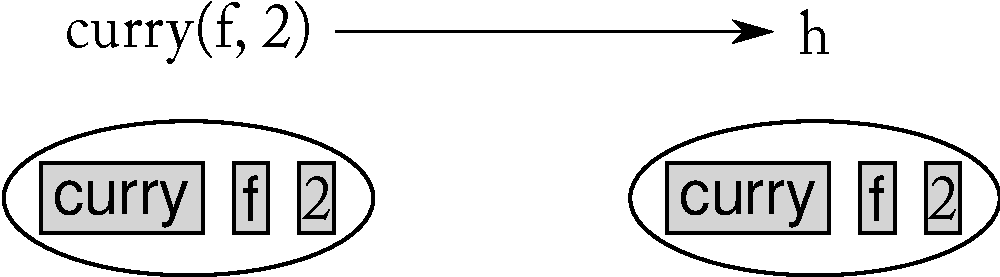
\includegraphics[height=60px]{curry1.pdf}

  \end{centering}

  \caption{Applying the \texttt{curry} function to a single argument $f$ produces a ``curried function'' $h$. The structure of $h$ is the same as the \encode that was evaluated.}
  \label{fig:curry1}
\end{figure}

\enlargethispage{3 \baselineskip}

\begin{figure}[h!]
  \begin{centering}
    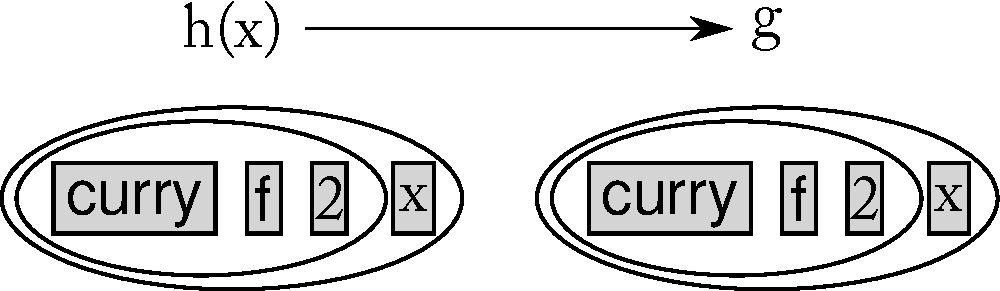
\includegraphics[height=60px]{curry2.pdf}

  \end{centering}

  \caption{Applying the $h$ function to an argument $x$ produces the new ``curried function'' $g$. The structure of $g$ is again the same as the \encode that was evaluated. Only
  when both arguments are available can the original $f$ function be invoked.}
  \label{fig:curry2}
\end{figure}

\begin{figure}[h!]
  \begin{centering}
    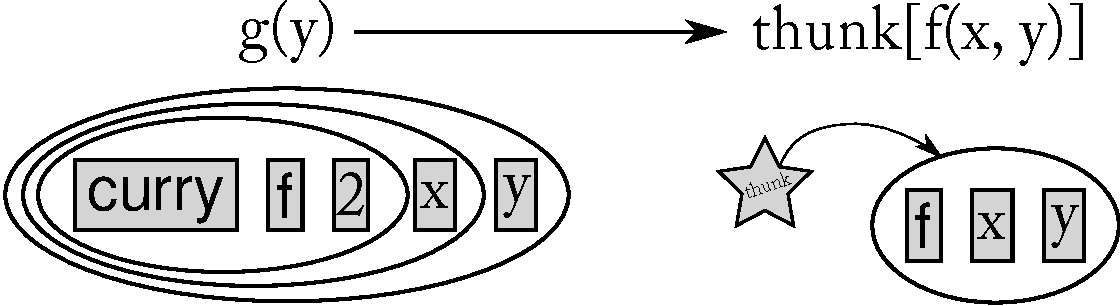
\includegraphics[height=60px]{curry3.pdf}

  \end{centering}

  \caption{Applying the $g$ function to an argument $y$ produces a \thunk for an \encode that computes $f(x, y)$.}
  \label{fig:curry3}
\end{figure}

\section{Open questions}

\begin{enumerate}[itemsep=0pt]
\item What is the latency overhead for a ``safe'' Wasm invocation, compared with a pure native function,
  and compared with forking a process on Linux?

\item What is the throughput overhead of running a C or C++ program
  that was compiled by \texttt{clang} into Wasm $\rightarrow$
  \texttt{wasm2c} $\rightarrow$ \texttt{libclang} $\rightarrow$
  \texttt{x86-64} ELF object, compared with compiling by \texttt{clang}
  directly into an \texttt{x86-64} ELF executable?

\item What should be the precise ``Fixpoint API'' exposed to Wasm via imported host functions that lets a function read the accessible \valuexs, create new \objects,
  create \trees that refer to recently created \objects, etc.?
  
\item What should be the additional API surface for an ``IO-Encode,'' e.g.~how to handle random numbers, time, filesystem and network access, user interaction?

\item How to implement the WASI API in a Wasm module, in terms of the Fixpoint API?
  
\item When/how to garbage-collect from the storage or memoization and trace caches?

\item How to share reproducible computations between users---perhaps by extending the Git on-disk format?
  
\item Execution strategy language separate from definition of a
  computation (to describe data placement / parallelization policy,
  garbage-collection policy, etc.)?
  
\item Does the approach to lazy inputs really ensure that a \thunk can
  always be replaced by (1) any other \thunk that refers to the same
  \valuex, or (2) the referred-to \valuex, without ever altering the
  result of a computation? (We don't want a function to be able to
  know if the runtime has or hasn't applied some optimization.) Does
  the system also successfully prevent cyclic references (e.g., two \thunks that resolve to
  each other)?

\item Can we run \texttt{clang.wasm} within Fixpoint, to compile
  \texttt{clang} into Wasm, to make the system self-hosting? Can we bootstrap an entire Linux distribution
  this way, perhaps following the Guix bootstrap dependency graph?

\item What's the right API for higher-level languages (e.g., Rust or C++) to expose constructs like, e.g.~a parallel map that compiles into an \encode with many inputs?

\item What should a ``visual debugger'' look like to inspect the computation flow and provenance of computed outputs?
  
\item \ldots
  
\end{enumerate}

\section{Commentary by Amit Levy (4/11/2021)}

In an attempt to understand the motivations behind some of the design
choices in the document, I've tried to recreate it from (sort of)
first-principles. This is useful for my own thought process but I also
believe that some of the non-obvious choices might actually be
important for answering some of the lingering questions you've
listed. Much of this is a restatement of what is in the doc, so
forgive the repetition. I'm also generalizing some, and specifying
other, assumptions about what types are returned by certain operations
because I couldn't really understand the reason behind the choices in
the design doc. However, I don't think these are important
distinctions. I've probably overlooked some detail or case but as far
as I can tell the changes are merely a simplification. Obviously,
please correct me if I'm wrong.

\bs

At a very high level, we want a system where computations are
reproducible (at least by default), that are trivially memoizable,
which are self-attesting, and which can take advantage of massive
burst parallelism. The core idea is represent both data and
computations as content-addressed objects.

\bs

At the very lowest level, as in git, all objects have values, that are
arbitrary vectors of bytes, and names that are cryptographic hashes of
the values. E.g.~Object.Name $leftarrow$ \textsc{sha256}(Object.Value)

\bs

Note that, so far, we do not need differentiate between ``Blobs''
``Trees'' ``Encodes'' etc. Similarly, git's storage layer does not
differentiate between trees, blobs, commits, etc. Instead, it's up to
the git ``plumbing'' layer to interpret values according to their
expected types. So: without considering computations, the only
operations we need in the system so far are:

\begin{itemize}
\item    get(Object.Name) $\rightarrow$ Object.Value
\item    put(Object.Value) $\rightarrow$ Object.Name
\end{itemize}
    
Ok, but we'd also like to include computations in this model. Very
much unlike git, these computations should be evaluated by the system
(rather than the user) in order to enable large-scale burst
parallelism. One simple way to add computation is to add a simple
``evaluate'' operation, that asks the system to execute some
computation---say Blob that happens to store executable Wasm. Let's
try to do this with as little change to the system as possible.

\bs

Evaluate takes a reference (object name) to a computation with zero
arguments (a thunk) that returns an object name (i.e. a 256-bit hash):
``() $\rightarrow$ Object.Name''. So now we have three operations:

\begin{itemize}
\item    get(Object.Name) $\rightarrow$ Object.Value
\item    put(Object.Value) $\rightarrow$ Object.Name
\item    evaluate(Object.Name) $\rightarrow$ Object.Name
\end{itemize}
  
To run a computation, we would first ``put'' it, then ``evaluate'' it
by reference, then ``get'' the result. A single evaluation always runs
in a single ``thread'' (for simplicity let's say a thread is tied to a
CPU thread, though I think enabling internal parallelism is probably
fine semantically and might be useful).

\bs

What is this computation permitted to do (in addition to normal
operations on local state such as registers, zero-initialized memory,
deterministic local file system, etc)? One option: it can perform
arbitrary gets, puts, evaluates.

\bs

This allows some indirection (by ``evaluating'' other thunks), and
allows the computation to return arbitrarily complex values (e.g., it
can construct a ``tree'' by performing a bunch of puts of blobs and
sub-trees, returning only the root of the tree), but does not give us
a way to write functions that accept arguments. This, in turn,
basically totally limits reuse.

\bs

Moreover, allowing arbitrary ``gets'' and ``evaluates'' within a
computation means the system would have to allow a computation to
block on I/O which\ldots well\ldots it seems bad\ldots we probably want to
avoid taking up resources unnecessarily, and we can avoid it. (Note
that puts from within the function need not result in blocking I/O,
since there is no need to externalize them until after the the thunk
is forced, so they can simply be stored locally in memory and
persistent at the end).

\bs

So, to get rid of ``get''s, we can simply add arguments to computations. As suggested, the notion of a closure/Encode, addresses this problem nicely:

\begin{verbatim}
// Rust pseudo-code for an Encode (Rust so I can express types concisely).
// `Object` and `Blob` both are actually SHA256 names, and the use of specific
// types just communicates which kinds of Objects are allowed/assumed to be in each field.
struct Encode {
  arguments: Vec<dyn Object>,
  function: Blob, // This blob needs to be WASM code
}
\end{verbatim}

Now, rather than allowing the function to perform arbitrary ``gets''
or ``evaluates,'' the function can refer, by index, to arguments that
are pre-fetched from the underlying store upon execution.

\bs

Implementing ``42 + 24'' is simple (if a bit overkill). The a user's perspective:

\bs

\begin{verbatim}
let a = put(42)
let b = put(24)

let addfunc = wasmc("return put(inputs[0] + inputs[1]);")
let add = put(addfunc)

let MyAddThunk = put(Encode {
  arguments: vec![a, b],
  function: add,
}

let aplusb = evaluate(MyAddThunk)
assert(get(aplusb) == 66)
\end{verbatim}

But now we can't do recursion and (sort of as a result) we can't
express parallel computations. While an Encode can construct (via
``puts'') and then return another Encode, it can't force the system to
evaluate it, since only users are permitted to call ``evaluate.''
Considering this is one of the main goals of the system, that's a
problem :).

\bs

There are at least two ways of addressing this---one way recursively
evaluates the results of Encodes until a fixpoint (look at that!)
while the other generates a computation DAG. I believe the system
described in the doc uses both of these methods. Notably, Nix/Guix
only use the former. I think there are important trade-offs here, so
this is maybe a big part of the meat of the design choices.

\bs

First the Nix/Guix approach. (Note: I'll use Nix to describe this
since I'm quite familiar with Nix and it's internals. It appears you
all are more familiar with Guix, which I have basically no familiarity
with beyond the documentation. I hope this isn't an issue as my
understanding is that Guix is simply a straightforward translation of
Nix from the the Nix expression language to Guile and that under the
hood their representations of derivations are equivalent, but I'm not
certain. So apologies in advance for any confusion this generates).

\bs

The key idea is to specify sub-computations, including recursive calls
to the same function, explicitly in the Encode---in Nix and Guix the
equivalent concept is called a derivation. In Nix, derivations have:

\begin{itemize}

\item    Input sources---these are references to blobs or tree (in Nix they are literally just paths in the nix store and can be either files or whole directories, but the point is they don't need to be evaluated)
\item Input derivations---these are references to other derivations who's values the current derivation depends on to compute. This tells Nix that before evaluating this derivation, the values of the input derivations had better be available. For example, most Nix derivations include the "bash" derivation in their input derivations since they (by default) use bash to run their builder script.
\item    Builder---this is sort of equivalent to ``function'' in Encodes. It's allowed to refer to a value that the output of one of the input derivations but can also itself be a value (e.g.~a blob that happens to be an executable).
\end{itemize}

The remaining fields in a Nix derivation (environment variables,
platform, and outputs) are sort of incidental, and not important for
this discussion, though worth thinking about for the next design
iteration since there may be some useful lessons about the
implementation details.

\bs

The encodes described in the design doc achieve something very similar
by separating lazy and strict inputs. Strict inputs may include other
encodes, which must be evaluated before evaluating the current Encode.

\bs

This structure has a number of benefits. It results in a
pre-determined computational DAG. By inspecting the derivations (or in
our case Encodes) recursively---which does not require actually
executing the Encodes---the system can generate a complete DAG,
determine an execution plan, execute dependencies in parallel etc.

\bs

Unsurprisingly (since this is the main goal of Nix/Guix), it's pretty
well suited for compiling code and its dependencies, structuring file
system heirarchies, etc. Example II in the design doc is a good
illustration of this. I believe anything that is basically a big
fan-out / fan-in works here.

\bs

One downside is that something needs to compute this DAG before
anything can actually be executed, and these DAGs can be reasonably
large. Perhaps computing the DAG can itself be an Encode somehow?
Idk\ldots

\bs

The second downside, is that we're limited to computations that can be totally unrolled. I.e., I don't believe we can compute fibonacci with using just these dependencies.

\bs

So, this is where the second method used in the design doc comes
in. Here, the system also forces whatever is returned from the
Encode. This means that an encode can produce an arbitrary,
data-dependent, new encode, return it, and it will be forced by the
system.

\bs

This is quite elegant and indeed can express any tail recursive computation (which, correct me if I'm wrong, is all computations). Awesome!

\bs

The main downside is that we can very easily end up with runaway
recursion and, in a potentially non-interactive system, we probably
need some way of dealing with this. It also potentially complicates
resource allocation since it means we don't have as much foresight
into what resources an Encode will use, how much parallelism, etc.

\bs

I also believe it complicates questions 6 \& 9. In Nix/Guix style
derivations, I believe the answers to these questions are relatively
straight forward, but with tail recursion garbage collection roots
seem trickier to define and I whether thunks can be cyclic is also
unclear to me.

\end{document}
